\begin{figure}[!bt]
  \begin{center}
    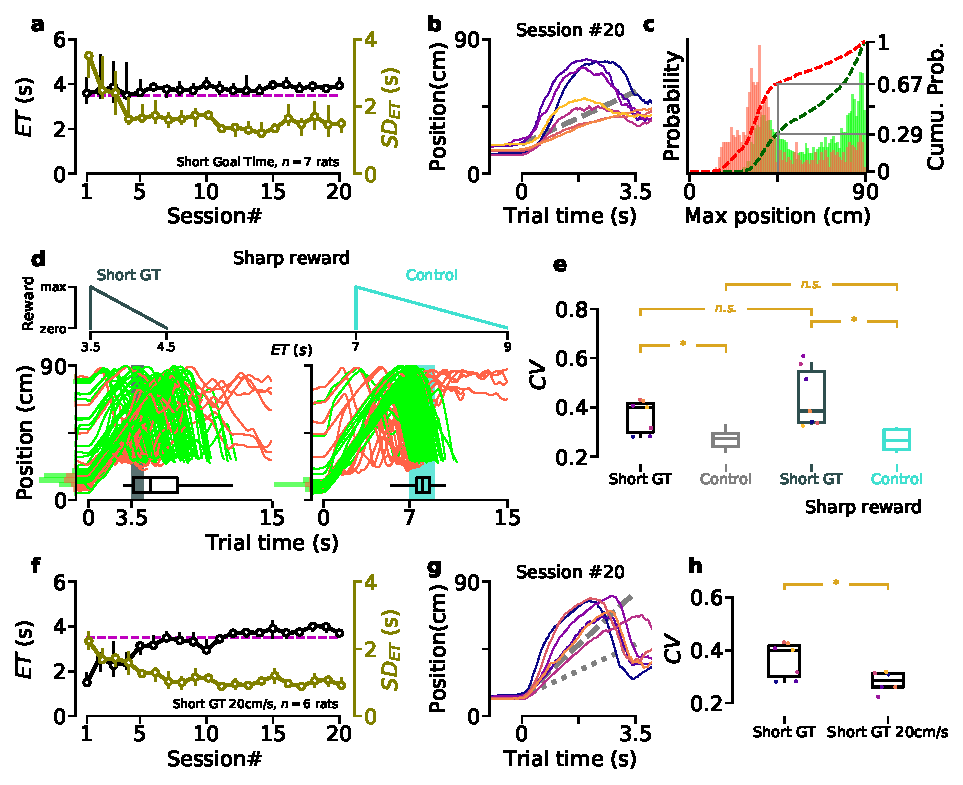
\includegraphics[width=\textwidth]{ch-time/figures/ShortGT-SharpTrd.pdf}
    \caption[Short~GT \& Sharp Conditions]
    {\textbf{Decreased temporal accuracy when the goal time is short.}
    \textbf{a)}
    Median $ET$ during training ($GT=3.5$~s).
    \textbf{b)}
    Median trajectory of ``short~GT'' animals after training.
    Colored lines indicate performance of individual animals.
    Dashed line's slope shows the treadmill speed (10~cm/s).
    \textbf{c)}
    PDF of the maximum position of the short~GT animals for correct (green) and error (red) trials.
    Dashed lines represent cumulative distributions (right y-axis).
    Data collected from session~\#~$\geq15$.
    \textbf{d)} 
    Sharp reward condition applied to short~GT and control experiments.
    \textit{Top}: reward profiles of the sharp reward condition applied to the short~GT (dark) and the control experiments (light).
    \textit{Bottom}: trajectories of 2 illustrative sessions after extensive training in sharp condition (\textit{left}, short~GT; \textit{right}, control).
    Highlighted areas indicate the reward window.
    \textbf{e)}
    Coefficient of variation~($CV$) for short~GT and control experiments with normal (the first two boxes), and sharp (the last two boxes) reward profiles.
    Data collected and averaged once performance plateaued.
    Short~GT vs. Control: $p<0.0001$;
    Sharp short~GT vs. Sharp control: $p<0.0001$.
    \textbf{f)}
    Similar to panel~a, for another group of animals trained to wait 3.5~s while the treadmill speed was 20~cm/s.
    \textbf{g)}
    Similar to panel~b, for animals of panel~f.
    Dashed line's slope shows the treadmill speed (20~cm/s).
    Dotted line's slope shows 10~cm/s.
    \textbf{h)}
    $CV$ for short~GT and short~GT at 20~cm/s conditions (same colors as in panels~b,~g).
    Data collected and averaged once performance plateaued.
    }
    \label{fig:time:shortSharp}
  \end{center}
\end{figure}